\documentclass[doublecol]{../macros/epl2} 
% or \documentclass[page-classic]{epl2} for one column style

\title{Measurement of proton-proton elastic scattering and total cross-section at $\sqrt s = 7\,\rm TeV$}
\shorttitle{Measurement of $\rm pp$ elastic scattering and total cross-section at $\sqrt s = 7\,\rm TeV$} %Insert here a short version of the title if it exceeds 70 characters

\author{%
The TOTEM Collaboration -- !! THIS IS JUST A PLACEHOLDER !! \\
G. Antchev\inst{(a)}, P. Aspell\inst{8}, I. Atanassov\inst{8,(a)}, V. Avati\inst{8}, J. Baechler\inst{8}, V. Berardi\inst{5b,5a},
G. Antchev\inst{(a)}, P. Aspell\inst{8}, I. Atanassov\inst{8,(a)}, V. Avati\inst{8}, J. Baechler\inst{8}, V. Berardi\inst{5b,5a},
G. Antchev\inst{(a)}, P. Aspell\inst{8}, I. Atanassov\inst{8,(a)}, V. Avati\inst{8}, J. Baechler\inst{8}, V. Berardi\inst{5b,5a},
G. Antchev\inst{(a)}, P. Aspell\inst{8}, I. Atanassov\inst{8,(a)}, V. Avati\inst{8}, J. Baechler\inst{8}, V. Berardi\inst{5b,5a},
G. Antchev\inst{(a)}, P. Aspell\inst{8}, I. Atanassov\inst{8,(a)}, V. Avati\inst{8}, J. Baechler\inst{8}, V. Berardi\inst{5b,5a},
G. Antchev\inst{(a)}, P. Aspell\inst{8}, I. Atanassov\inst{8,(a)}, V. Avati\inst{8}, J. Baechler\inst{8}, V. Berardi\inst{5b,5a},
G. Antchev\inst{(a)}, P. Aspell\inst{8}, I. Atanassov\inst{8,(a)}, V. Avati\inst{8}, J. Baechler\inst{8}, V. Berardi\inst{5b,5a},
G. Antchev\inst{(a)}, P. Aspell\inst{8}, I. Atanassov\inst{8,(a)}, V. Avati\inst{8}, J. Baechler\inst{8}, V. Berardi\inst{5b,5a},
G. Antchev\inst{(a)}, P. Aspell\inst{8}, I. Atanassov\inst{8,(a)}, V. Avati\inst{8}, J. Baechler\inst{8}, V. Berardi\inst{5b,5a},
G. Antchev\inst{(a)}, P. Aspell\inst{8}, I. Atanassov\inst{8,(a)}, V. Avati\inst{8}, J. Baechler\inst{8}, V. Berardi\inst{5b,5a},
G. Antchev\inst{(a)}, P. Aspell\inst{8}, I. Atanassov\inst{8,(a)}, V. Avati\inst{8}, J. Baechler\inst{8}, V. Berardi\inst{5b,5a},
G. Antchev\inst{(a)}, P. Aspell\inst{8}, I. Atanassov\inst{8,(a)}, V. Avati\inst{8}, J. Baechler\inst{8}, V. Berardi\inst{5b,5a},
G. Antchev\inst{(a)}, P. Aspell\inst{8}, I. Atanassov\inst{8,(a)}, V. Avati\inst{8}, J. Baechler\inst{8} \and V. Berardi\inst{5b,5a}
%\thanks{bla}
}

\shortauthor{G.~Atchev \etal}

\institute{%
	\inst{1a} Institute of Physics of the Academy of Sciences of the Czech Republic - Praha, Czech Republic, EU\\
	\inst{1b} Czech Technical University - Praha, Czech Republic, EU\\
	\inst{2} National Institute of Chemical Physics and Biophysics NICPB Tallinn, Estonia, EU\\
	\inst{3a} Helsinki Institute of Physics - Helsinki, Finland, EU\\
	\inst{3b} Department of Physics, University of Helsinki - Helsinki, Finland, EU\\
	\inst{4} MTA KFKI RMKI - Budapest, Hungary, EU\\
	\inst{5a} INFN Sezione di Bari - Bari, Italy, EU\\
	\inst{5b} Dipartimento Interateneo di Fisica di Bari - Bari, Italy, EU\\
	\inst{6a} Sezione INFN di Genova - Genova, Italy, EU\\
	\inst{6b} Universit\` a degli Studi di Genova - Genova, Italy, EU\\
	\inst{7a} INFN Sezione di Pisa - Pisa, Italy, EU\\
	\inst{7b} Universit\` a degli Studi di Siena and Gruppo Collegato INFN di Siena - Siena, Italy, EU\\
	\inst{8} CERN - Geneva, Switzerland\\
	\inst{9} Case Western Reserve University, Department of Physics - Cleveland, OH, USA\\
	\inst{10} Penn State University, Department of Physics - University Park, PA, USA
}

\pacs{13.60.Hb}{Total and inclusive cross sections (including deep-inelastic processes)}


\abstract{%
!! THIS IS JUST A PLACEHOLDER !!\\
TOTEM has measured the differential cross-section for elastic proton-proton scattering
at the LHC energy of √
s = 7 TeV analysing data from a short run with dedicated large-β∗ optics.
A single exponential fit with a slope B = (20.1 0.2stat 0.3syst ) GeV−2 describes the range of the
± ±four-momentum transfer squared from 0.02 to 0.33 GeV2. After the extrapolation to = 0,
|t| |t|a total elastic scattering cross-section of (24.8 0.2stat 1.2syst) mb was obtained. Applying
± ±the optical theorem and using the luminosity measurement from CMS, a total proton-proton
cross-section of (98.3 0.2stat 2.8syst) mb was deduced which is in good agreement with the
± ±expectation from the overall fit of previously measured data over a large range of center-of-mass
energies. From the total and elastic pp cross-section measurements, an inelastic pp cross-section
of (73.5 0.6stat +1.8
 syst) mb was inferred.
± −1.3
}


\def\d{{\rm d}}
\def\un#1{\,{\rm #1}}
\def\ung#1{\quad[{\rm #1}]}
\def\unt#1{[{\rm #1}]}
\def\e{{\rm e}}

\setbox123\hbox{\small$0$}
\def\S{\hbox to\wd123{\hss}}
\setbox124\hbox{\small$_{0}$}
\def\s{\hbox to\wd124{\hss}}


\begin{document}

\maketitle

%--------------------------------------------------
\section{Introduction}

TODO: Explain context of this paper, relation to papers 2 and 3.

TODO: Here, we used luminosity from CMS, lumi-independent results will come in paper 3.

TODO: Describe TOTEM - RP, T1, T2; Here only elastic scattering -- only RP -- bridge to the next chapter.


%--------------------------------------------------
\section{Proton measurement with Roman Pots}

\subsection{Roman Pot system}

TODO: Describe the system of RPs: stations, units, ...

TODO: The measurement is performed with the vertical RPs in $220\un{m}$ stations only -- the concept of two diagonals

\subsection{Optics}

Elastic proton transport for $\beta^* = 90\un{m}$ optics:

\begin{equation}
\label{transport}
x^{\rm N} = L_x\,\theta^*_x + v_x\,x^*\ ,\ 
x^{\rm F} = v_x\,x^*\ ,\ 
y = L_y\,\theta^*_y + v_y\,y^*
\end{equation}


TODO: brief description of optics, refer to \cite{epl96} where details are discussed

TODO: define $\xi$

Kinematics reconstruction from one-arm measurement:
\begin{equation}
\label{reconstruction}
x^* = {x^{\rm F}\over v_x}\ ,\quad
\theta^*_x = {1\over {\d L_x\over \d s}} \left( \theta_x - {\d v_x\over \d s} x^* \right)\ ,\quad
\theta^*_y = {y\over L_y}\ .
\end{equation}

For elastic events, we averaged the angles reconstructed from left and right arms, which further reduces the uncertainty.

%--------------------------------------------------
\section{Data taking}

The presented date were recorded during fill 2232 on 10 October 2011, using $\beta^* = 90\un{m}$ optics. For this analysis, only one bunch-pair was used (with populations $5\cdot10^{10}$ and $6\cdot10^{10}$ protons). This bunch-pair produced an instantaneous luminosity dropping from about $6.9$ to $4.3\un{mb^{-1} s^{-1}}$ during the run.

Several trigger schemes were used in the data-taking. For this analysis, the essential one was the RP trigger -- requiring a track-segment in any of the RPs, in at least one of the transverse projections $u$ and $v$, but simultaneously at both arms of the experiment. In order to determine various efficiency corrections, we profited from a zero-bias trigger -- triggering on random bunch-crossings. 

During the run, the Roman Pots (RPs) were driven to three different distances from the beam -- see Tab.~\ref{datasets}. While most of the statistics falls into the first dataset, the other two allowed us to measure $|t|$ values down to $4.6\cdot10^{-3}\un{GeV^2}$. Having three different datasets has enabled us to quantify and reduce certain systematic uncertainties.

\begin{table}
\caption{Description of the three datasets available. The RP position gives the RP approach to beam in multiples of the beam size ($\sigma_{\rm beam}$). The third column summarizes the numbers of elastic events reconstructed from both diagonals. The $\mathcal{L}_{\rm eff}$ gives the effective (taking into account the DAQ efficiency) luminosity for each dataset. The last column shows the lowest $|t|$ values reached.}
\label{datasets}
\begin{center}
\vskip-3mm
\begin{tabular}{ccccc}\hline
& RP & elastic                   & $\mathcal{L}_{\rm eff}$ & $|t|_{\rm min}$     \cr
\omit\hss\vbox to 0pt{\vss\hbox{\ dataset\ }\vss}\hss &\multispan4 \cr
 &  position &  events                   & $\unt{mb^{-1}}$         & $\unt{GeV^2}$       \cr\hline
1 & $6.5\,\sigma_{\rm beam}$ & 841k      & $68.2$                  & $7.3\cdot10^{-3}$ \cr
2 & $5.5\,\sigma_{\rm beam}$ & 106k      & $8.2$                   & $5.7\cdot10^{-3}$ \cr
3 & $4.8\,\sigma_{\rm beam}$ & 89k       & $6.6$                   & $4.6\cdot10^{-3}$ \cr\hline
\end{tabular}
\end{center}
\end{table}


%--------------------------------------------------
\section{Analysis}

The analysis is very similar the one of \cite{epl96}. Before describing the steps, let us anticipate that all datasets were analyzed separately. Moreover, most of the steps are performed independently for the two diagonals. In this way, we gained a better control of the systematics.

%-------------------------
\subsection{Alignment}

Three complementary methods were applied. First, the RP motor control was calibrated in a beam-touching exercise. Then, proton tracks passing through the overlap between vertical and horizontal RPs were used to determine the relative alignment among the RPs of each unit. Since the elastic event tagging does not require precise alignment, we could use an elastic pre-selection for alignment fine-tuning. By exploiting the azimuthal symmetry of elastic scattering and taking advantage of the very small effective length $L_x$, we could adjust the horizontal and vertical shifts and the tilt of each unit. The effect of residual misalignments on $\d\sigma_{\rm el}/\d t$ was thus smaller than $0.3\%$ for every $t$-bin.

%-------------------------
\subsection{Elastic tagging}

The cuts used to select the elastic events are summarized in Tab.~\ref{cuts}. The cuts 1 and 2 require the reconstructed track collinearity between the left and right arms. The cuts 3-6 effectively work as low-$\xi$ cuts. If $\xi$ is non-negligible, the vertex ($x^*$) reconstruction Eq.~\ref{reconstruction} is broken. So is the correlation between the track position ($y^{\rm N}$) and the track angle (proportional to $y^{\rm F} - y^{\rm N}$). The cut 7 compares the horizontal vertex position reconstructed from the left and right arms. It is the strongest single cut and is very effective against the beam-halo background, see Fig.~\ref{hit dist}.

\begin{table}
\caption{The elastic selection cuts. The superscripts R and L refer to the right and left arm, the N and F corresponds to the near and far units. TODO: threshold = 1 sigma, cuts applied at 3 sigma}
\label{cuts}
\begin{center}
\begin{tabular}{ccc}\hline
number & cut & threshold\cr\hline
diagonal &\multispan2 \hss track reconstructed in all 4 diagonal RPs \hss \cr
1 & $\theta_x^{*\rm R}$ vs. $\theta_x^{*\rm L}$		& $9.2\un{\mu rad}$	\cr
2 & $\theta_y^{*\rm R}$ vs. $\theta_y^{*\rm L}$		& $3.5\un{\mu rad}$	\cr
3 & $|x^{*\rm R}|$ 									& $200\un{\mu m}$	\cr
4 & $|x^{*\rm L}|$ 									& $200\un{\mu m}$	\cr
5 & $y^{\rm R,N}$ vs.~$y^{\rm R,F} - y^{\rm R,N}$	& $17\un{\mu m}$	\cr
6 & $y^{\rm R,N}$ vs.~$y^{\rm L,F} - y^{\rm L,N}$	& $17\un{\mu m}$	\cr
7 & $x^{*\rm R}$ vs. $x^{*\rm L}$					& $9\un{\mu m}$ 	\cr\hline
\end{tabular}
\end{center}
\end{table}


%-------------------------
\subsection{Kinematics reconstruction}

The scattering angles were reconstructed according to Eq.~\ref{reconstruction}. The optics uncertainties for (one-arm) $\theta^*_x$ and $\theta^*_y$ reconstruction were $1.3\%$ and $0.8\%$ respectively. The former one has a more pronounced effect on $\d\sigma_{\rm el}/\d t$ (due to higher value and no acceptance cut in $\theta^*_x$) and is the leading systematic uncertainty for larger $|t|$ values, cf.~Tab.~\ref{systematics}.


%-------------------------
\subsection{Background}

The background contribution (i.e.~all non-elastic events passing the selection cuts) was estimated by relaxing the strongest single cut (number 7 in Tab.~\ref{cuts}) and analyzing the distribution of $x^{*\rm R} - x^{*\rm L}$. This distribution can reasonably be described by two Gaussians -- one for the signal and for the background. We determined the background/signal ratio to be $(0.8 \pm 0.4)\%$.


%-------------------------
\subsection{Acceptance correction}

We identified two acceptance limitations: the detector edge (relevant for lower $|t|$) and the LHC aperture limitation shown in Fig.~\ref{hit dist} right (relevant for higher $|t|$). Both effects were treated by assuming azimuthal symmetry of the elastic scattering and by correcting for smearing around the limitation edges. In order to keep the uncertainty on a reasonable level, we constrained ourselves to the region where the full acceptance correction was no larger than 7.5 (considering both diagonals).


%-------------------------
\subsection{Unfolding of resolution effects}

The angular resolution was determined by comparing the scattering angles reconstructed from the left and right arm. Combining all three datasets and all diagonals yields one-arm resolutions $(6.36\pm 0.21)\un{\mu rad}$ in $\theta^*_x$ and $(2.47\pm 0.07)\un{\mu rad}$ in $\theta^*_y$. The latter one is predominantly given by the beam-divergence, the $\theta^*_x$ resolution is deteriorated by a contribution from the finite detector pitch.

The $t$-resolution impact on $\d\sigma_{\rm el}/\d t$  was determined (and eliminated) by an iterative procedure. That starts by taking the observed (smeared) $t$-distribution as an input to a Monte-Carlo calculation of the un-smearing correction. The correction is applied to the observed $t$-distribution which yields a better estimate of the true $t$-distribution. These two steps were repeated three times in total. The systematic uncertainty of this procedure (due to the uncertainty of the $\theta^*_{x, y}$ resolution) was estimated smaller than $0.5\%$.

%-------------------------
\subsection{Efficiencies}

The efficiency of the RP trigger was estimated using the zero-bias data stream. We repeated the elastic event selection on these data and found the RP trigger efficient for all the selected events. Therefore, on $68\%$ confidence level, we concluded the trigger efficiency to be higher than $99.8\%$.
% 95% CL: 99.40

The DAQ efficiency was determined by comparing the numbers of triggered and recorded events, yielding $(98.142 \pm 0.001)\%$.

There are several reasons for reconstruction inefficiency: intrinsic RP detection inefficiency of each silicon sensor, proton interaction with the material of a RP and ``pile-up'' of several protons in one event (RPs can fully reconstruct at most one track). For the last case, the most important situation is a coincidence of an elastic proton and a beam-halo proton, see Fig.~\ref{hit dist}.

Uncorrelated inefficiencies of single RPs were studied by removing the examined RP from the selection cuts (only cut 2 can be kept then) and counting the recuperated events. The result of this study was an inefficiency of $(1.5 \pm 0.2)\%$ for the near and $(3.0 \pm 0.2)\%$ for the far RPs. This difference can be explained by proton interactions in the near pot that affect the far RP too. This near-far correlated inefficiency was determined from data by counting events with corresponding shower signatures, yielding $(1.5\pm 0.7)\%$.
% confirmation from MC simulations.

The ``pile-up'' inefficiency was determined from the zero-bias data stream by evaluating the probability of finding a track in both RPs on either side. This probability was found increasing as RPs approached the beam. For instance, for the diagonal bottom-left top-right, the probabilities were $(3.9 \pm 0.3)\%$, $(6.2 \pm 0.3)\%$ and $(7.9 \pm 0.3)\%$ for the datasets 1, 2 and 3 respectively.


\begin{figure*}
\begin{center}
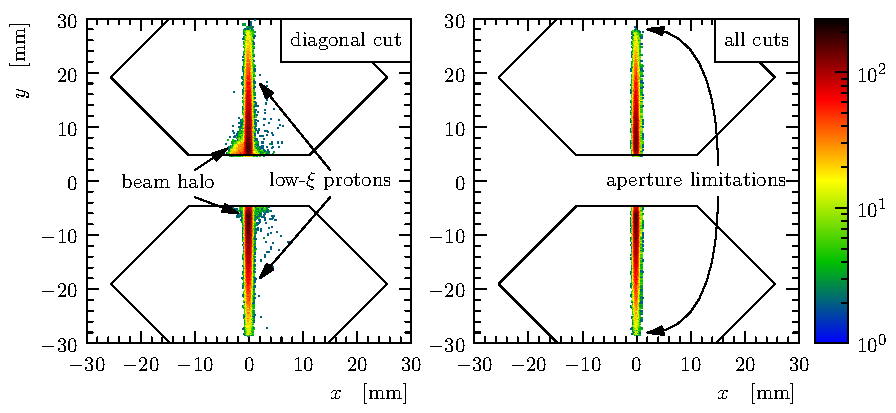
\includegraphics{fig/hit_dist.pdf}
\vskip-5mm
\caption{Hit distributions from dataset 3 in the far unit of the $220\un{m}$ station, right arm. Left: with diagonal cut only, Right: with all the elastic selection cuts (see Tab.~\ref{cuts}). The left plot clearly indicates the presence of the beam halo, which is eliminated by the selection cuts (the right plot). The distribution of elastic hits in right plot is sharply cut at about $|y| = 29\un{mm}$ which is a consequence of the LHC aperture limitations. }
\label{hit dist}
\end{center}
\end{figure*}

%-------------------------
\subsection{Luminosity}

TODO: Lumi from CMS, 4\% uncertainty, Ken's pedestal subtraction

\subsection{Extrapolation to $t=0\,\rm GeV^2$}

The elastic differential cross section was extrapolated to zero with the following parameterization:
\begin{equation}
\label{extrapolation}
{\d\sigma_{\rm el}\over \d t} = \left. {\d\sigma_{\rm el}\over \d t}\right|_{t=0} \ \e^{-B|t|}\ .
\end{equation}
The fits were performed from the lowest accessible $|t|$ values (see $|t|_{\rm min}$ in Tab.~\ref{datasets}) to $|t| = 0.2\un{GeV^2}$, with a typical $\chi^2/\hbox{n.d.f.}$ of $1.2$ -- see for example the green line in Fig.~\ref{dsdt}.

%-------------------------
\section{Systematic uncertainty calculation}

%TODO: Statistical uncertainty negligible, see Tab.~\ref{results}.

For each of the analysis steps above, the systematic uncertainty was determined, and their combination was studied with a Monte-Carlo simulation. We treated separately analysis $t$-dependent, analysis $t$-independent (normalization) and luminosity uncertainties, the results are shown in Tab.~\ref{systematics}. Since there is a number of contributions in each category, we combined the uncertainties in quadrature. So we did for the total uncertainty.

The luminosity uncertainty is the leading systematic effect for $|t| < 0.2\un{GeV^2}$, above that it is the uncertainty of $\d L_x/\d s$ which dominates. The optics-related error contribution is almost vanishing around $|t| = 0.06\un{GeV^2}$ and has opposite signs left and right of that point. Therefore there is a partial error cancellation in the integrated elastic cross section. Consequently the relative error of $\sigma_{\rm el}$ is significantly lower than the one of $\d\sigma_{\rm el}/\d t|_0$ -- see Tab.~\ref{results}.

The Monte-Carlo simulation confirms that there is a strong correlation between the errors of $\sigma_{\rm el}$ and $\d\sigma_{\rm el}/\d t|_0$ -- the correlation coefficient is $0.76$ (when both $t$-dependent and normalization contributions are included).

\begin{largetable}
\caption{Overview of systematic uncertainties}
%\vskip-3mm
\label{systematics}
\begin{tabular}{cccccccccc}\hline
$t\ung{GeV^2}$ &	0.005 &	0.01 &	0.06 &	0.1 &	0.12 &	0.16 &	0.2 &	0.3 &	0.4\cr\hline
$t$-dependent &	1.8\% &	1.0\% &	0.3\% &	0.9\% &	1.2\% &	3.0\% &	4.4\% &	8.3\% &	12.3\%\cr
normalization &\multispan9\hfil	1.2\%\hfil  \cr
luminosity &\multispan9\hfil	4.0\%\hfil  \cr\hline
total &	4.5\% &	4.3\% &	4.2\% &	4.3\% &	4.3\% &	5.1\% &	6.1\% &	9.3\% &	12.9\% \cr\hline

\end{tabular}
\end{largetable}


%--------------------------------------------------
\section{Results}

The differential cross section results obtained from different datasets and different diagonals match perfectly with each other and with our previous publication \cite{epl95}. Merging the data from all datasets and diagonals gives the differential cross section presented in Fig.~\ref{dsdt} and Tab.~\ref{data low t}. Let us note that the first (second) lowest $|t|$ bin comes from the dataset 3 (datasets 2 and 3) only -- that is why these bins have significantly higher statistical uncertainty.

Tab.~\ref{data low t} gives a representative $t$ value for each bin. These points were determined from the requirement that bin-based and point-based $\chi^2$ minimizations would lead to identical results \cite{lafferty94}. In practice, each bin $B_i$ of width $w_i$ is represented by $t_i$ value that fulfils $f(t_i) = {1\over w_i} \int_{B_i} f(\tau)\, \d\tau$, where $f(t)$ stands for the $t$-distribution. The uncertainties of the representative points $t_i$ come from the uncertainty of the $f(t)$ determination (fit). Even considering both statistical (bin fluctuations) and systematic (different fit parameterizations) gives negligible uncertainties on the representative $t$-values (relative uncertainties smaller than $10^{-4}$).

Tab.~\ref{data medium t} gives the $\d\sigma_{\rm el}/\d t$ continuation to higher $|t|$ values, measured with $\beta^* = 3.5\un{m}$ optics and published in \cite{epl95}.

%\begin{figure*}
%\begin{center}
%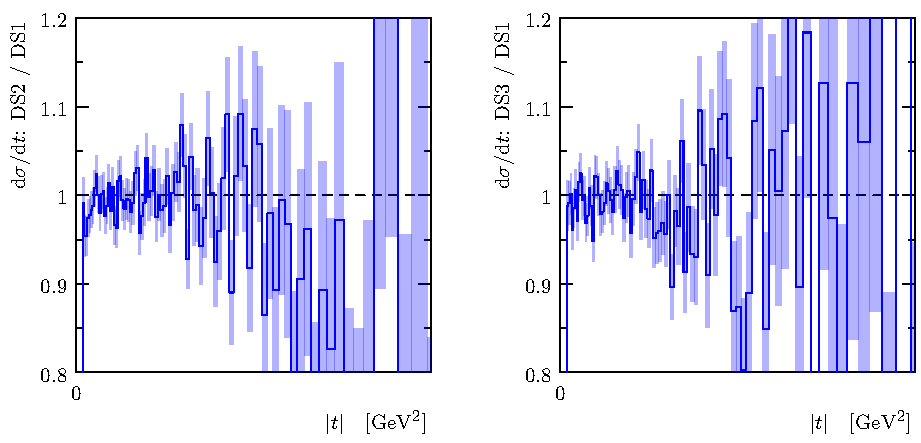
\includegraphics{fig/dsdt_dataset_ratio.pdf}
%\caption{A figure that demonstrates the excelent match between the data-sets.}
%\label{f.lbl}
%\end{center}
%\end{figure*}

\begin{figure*}
\begin{center}
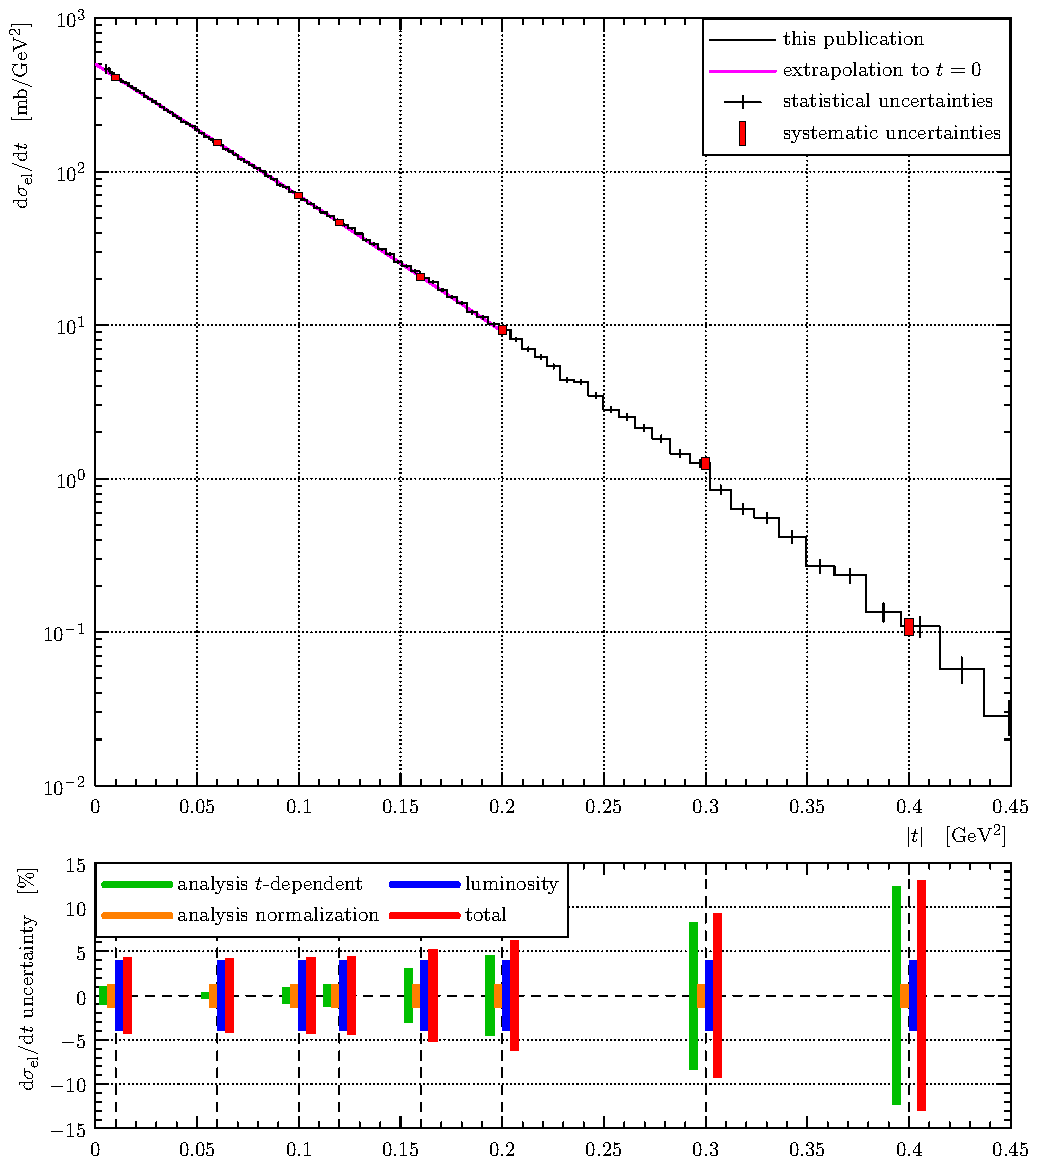
\includegraphics{fig/dsdt.pdf}
\caption{The measured elastic differential cross section. TODO: more description?}
\label{dsdt}
\end{center}
\end{figure*}

\setlength{\tabcolsep}{3.8pt}

\begin{largetable}
\caption{The elastic differential cross section determined in this analysis. Some details on the systematic uncertainty calculation can be found in Tab.~\ref{systematics}. That table can also be used to evaluate the correlations of the systematic uncertainties among the bins (the three contributions are independent).}
\label{data low t}
\begin{center}
%\vskip-3mm
\small
\begin{tabular}{cc@{$\pm$}c@{$\pm$}cccc@{$\pm$}c@{$\pm$}cccc@{$\pm$}c@{$\pm$}cccc@{$\pm$}c@{$\pm$}c}
\multispan4\hrulefill&&\multispan4\hrulefill&&\multispan4\hrulefill&&\multispan4\hrulefill\cr
$|t|$ & \multispan3\hss$\d \sigma_{\rm el}/\d t \ung{\mu b/GeV^2}$\hss&&
$|t|$ & \multispan3\hss$\d \sigma_{\rm el}/\d t \ung{\mu b/GeV^2}$\hss&&
$|t|$ & \multispan3\hss$\d \sigma_{\rm el}/\d t \ung{\mu b/GeV^2}$\hss&&
$|t|$ & \multispan3\hss$\d \sigma_{\rm el}/\d t \ung{\mu b/GeV^2}$\hss
\cr
$\unt{GeV^2}$ &&stat&syst&&
$\unt{GeV^2}$ &&stat&syst&&
$\unt{GeV^2}$ &&stat&syst&&
$\unt{GeV^2}$ &&stat&syst
\cr
\multispan4\hrulefill&&\multispan4\hrulefill&&\multispan4\hrulefill&&\multispan4\hrulefill\cr
$0.00515$ & $465.\S$ & $27.\S$ & $21.\S$ && $0.0499$ & $187.5\S$ & $1.3\S$ & $7.9\S$ && $0.112$ & $54.11$ & $0.53$ & $2.33$ && $0.213$ & $6.98\S\S$ & $0.19\S\S$ & $0.45\S\S$ \cr
$0.00650$ & $465.\S$ & $11.\S$ & $21.\S$ && $0.0522$ & $178.1\S$ & $1.2\S$ & $7.5\S$ && $0.116$ & $51.21$ & $0.51$ & $2.20$ && $0.219$ & $6.22\S\S$ & $0.17\S\S$ & $0.42\S\S$ \cr
$0.00818$ & $437.5$ & $\S5.0$ & $19.1$ && $0.0545$ & $168.8\S$ & $1.2\S$ & $7.1\S$ && $0.119$ & $48.24$ & $0.49$ & $2.07$ && $0.225$ & $5.38\S\S$ & $0.16\S\S$ & $0.37\S\S$ \cr
$0.00995$ & $411.0$ & $\S3.3$ & $17.7$ && $0.0569$ & $162.5\S$ & $1.1\S$ & $6.8\S$ && $0.122$ & $44.99$ & $0.46$ & $1.96$ && $0.232$ & $4.40\S\S$ & $0.14\S\S$ & $0.31\S\S$ \cr
$0.0117\S$ & $402.3$ & $\S2.9$ & $17.3$ && $0.0592$ & $155.5\S$ & $1.1\S$ & $6.5\S$ && $0.126$ & $42.74$ & $0.45$ & $1.89$ && $0.239$ & $4.25\S\S$ & $0.14\S\S$ & $0.31\S\S$ \cr
$0.0135\S$ & $384.5$ & $\S2.6$ & $16.5$ && $0.0616$ & $149.4\S$ & $1.1\S$ & $6.3\S$ && $0.130$ & $39.49$ & $0.43$ & $1.77$ && $0.246$ & $3.47\S\S$ & $0.13\S\S$ & $0.26\S\S$ \cr
$0.0154\S$ & $378.0$ & $\S2.4$ & $16.2$ && $0.0641$ & $140.2\S$ & $1.0\S$ & $5.9\S$ && $0.133$ & $35.75$ & $0.43$ & $1.63$ && $0.253$ & $2.82\S\S$ & $0.11\S\S$ & $0.22\S\S$ \cr
$0.0172\S$ & $360.3$ & $\S2.3$ & $15.4$ && $0.0666$ & $135.10$ & $0.99$ & $5.70$ && $0.137$ & $33.63$ & $0.41$ & $1.56$ && $0.261$ & $2.52\S\S$ & $0.10\S\S$ & $0.20\S\S$ \cr
$0.0191\S$ & $348.1$ & $\S2.2$ & $14.9$ && $0.0691$ & $129.00$ & $0.96$ & $5.45$ && $0.141$ & $31.08$ & $0.41$ & $1.47$ && $0.270$ & $2.142\S$ & $0.097\S$ & $0.178\S$ \cr
$0.0210\S$ & $337.0$ & $\S2.1$ & $14.4$ && $0.0716$ & $120.53$ & $0.91$ & $5.10$ && $0.145$ & $28.91$ & $0.39$ & $1.39$ && $0.278$ & $1.824\S$ & $0.086\S$ & $0.157\S$ \cr
$0.0229\S$ & $325.0$ & $\S2.0$ & $13.9$ && $0.0742$ & $115.10$ & $0.89$ & $4.88$ && $0.149$ & $25.65$ & $0.38$ & $1.25$ && $0.287$ & $1.455\S$ & $0.075\S$ & $0.129\S$ \cr
$0.0248\S$ & $307.9$ & $\S1.9$ & $13.1$ && $0.0769$ & $109.63$ & $0.86$ & $4.65$ && $0.153$ & $24.16$ & $0.36$ & $1.20$ && $0.297$ & $1.257\S$ & $0.069\S$ & $0.116\S$ \cr
$0.0268\S$ & $296.7$ & $\S1.8$ & $12.7$ && $0.0795$ & $104.97$ & $0.83$ & $4.46$ && $0.157$ & $22.35$ & $0.35$ & $1.13$ && $0.307$ & $0.848\S$ & $0.055\S$ & $0.081\S$ \cr
$0.0287\S$ & $285.9$ & $\S1.8$ & $12.2$ && $0.0823$ & $100.22$ & $0.80$ & $4.27$ && $0.162$ & $20.22$ & $0.34$ & $1.04$ && $0.318$ & $0.633\S$ & $0.046\S$ & $0.063\S$ \cr
$0.0307\S$ & $275.3$ & $\S1.7$ & $11.7$ && $0.0850$ & $\S93.18$ & $0.76$ & $3.97$ && $0.166$ & $19.01$ & $0.32$ & $1.00$ && $0.330$ & $0.558\S$ & $0.043\S$ & $0.058\S$ \cr
$0.0328\S$ & $263.0$ & $\S1.6$ & $11.2$ && $0.0878$ & $\S89.16$ & $0.74$ & $3.81$ && $0.171$ & $16.92$ & $0.30$ & $0.91$ && $0.342$ & $0.417\S$ & $0.038\S$ & $0.045\S$ \cr
$0.0348\S$ & $252.0$ & $\S1.6$ & $10.7$ && $0.0907$ & $\S81.78$ & $0.70$ & $3.50$ && $0.175$ & $15.20$ & $0.29$ & $0.83$ && $0.356$ & $0.269\S$ & $0.027\S$ & $0.030\S$ \cr
$0.0369\S$ & $242.8$ & $\S1.5$ & $10.3$ && $0.0936$ & $\S78.85$ & $0.68$ & $3.38$ && $0.180$ & $13.90$ & $0.28$ & $0.78$ && $0.371$ & $0.235\S$ & $0.025\S$ & $0.028\S$ \cr
$0.0390\S$ & $231.6$ & $\S1.5$ & $\S9.8$ && $0.0966$ & $\S73.92$ & $0.65$ & $3.17$ && $0.185$ & $12.09$ & $0.26$ & $0.69$ && $0.387$ & $0.136\S$ & $0.019\S$ & $0.017\S$ \cr
$0.0411\S$ & $222.2$ & $\S1.4$ & $\S9.4$ && $0.0996$ & $\S68.77$ & $0.62$ & $2.96$ && $0.190$ & $11.26$ & $0.25$ & $0.66$ && $0.405$ & $0.109\S$ & $0.016\S$ & $0.014\S$ \cr
$0.0433\S$ & $210.9$ & $\S1.4$ & $\S8.9$ && $0.103\S$ & $\S65.53$ & $0.60$ & $2.82$ && $0.196$ & $10.11$ & $0.23$ & $0.61$ && $0.425$ & $0.0575$ & $0.0110$ & $0.0079$ \cr
$0.0455\S$ & $204.8$ & $\S1.3$ & $\S8.7$ && $0.106\S$ & $\S61.90$ & $0.58$ & $2.66$ && $0.201$ & $\S9.31$ & $0.22$ & $0.57$ && $0.448$ & $0.0285$ & $0.0072$ & $0.0042$ \cr
\multispan4&&\multispan4&&\multispan4&&\multispan4\hrulefill\cr
$0.0477\S$ & $197.2$ & $\S1.3$ & $\S8.3$ && $0.109\S$ & $\S58.11$ & $0.55$ & $2.50$ && $0.207$ & $\S8.07$ & $0.21$ & $0.51$ \cr
\multispan4\hrulefill&&\multispan4\hrulefill&&\multispan4\hrulefill&\cr
\end{tabular}
\end{center}
\end{largetable}


\begin{largetable}
\caption{The elastic differential cross section as determined in \cite{epl95}. The systematic errors almost fully correlated among the bins.
%systematic uncertainties evaluated for three $|t|$ values: $^{+25}_{-37}\%$ at $|t|=0.4\un{GeV^2}$, $^{+28}_{-39}\%$ at $0.5\un{GeV^2}$ and $^{+27}_{-30}\%$ at $1.5\un{GeV^2}$.
}
\label{data medium t}
\begin{center}
%\vskip-3mm
\small
\begin{tabular}{c@{$\pm$}cc@{$\pm$}c@{$\pm$}ccc@{$\pm$}cc@{$\pm$}c@{$\pm$}ccc@{$\pm$}cc@{$\pm$}c@{$\pm$}c}
\multispan5\hrulefill&&\multispan5\hrulefill&&\multispan5\hrulefill\cr
\multispan2\hss $|t| \ung{GeV^2}$\hss & \multispan3\hss$\d \sigma_{\rm el}/\d t \ung{\mu b/GeV^2}$\hss&&
\multispan2\hss $|t| \ung{GeV^2}$\hss & \multispan3\hss$\d \sigma_{\rm el}/\d t \ung{\mu b/GeV^2}$\hss&&
\multispan2\hss $|t| \ung{GeV^2}$\hss & \multispan3\hss$\d \sigma_{\rm el}/\d t \ung{\mu b/GeV^2}$\hss\cr
\multispan2&&stat&syst&&
\multispan2&&stat&syst&&
\multispan2&&stat&syst\cr
\multispan5\hrulefill&&\multispan5\hrulefill&&\multispan5\hrulefill\cr
$0.3642$ & $0.0019$ & $299.1\S$ & $7.6\S$ & $^{\s71.6\s}_{108.5\s}$ & & $0.6434$ & $0.0041$ & $24.65$ & $0.99$ & $^{\s6.87}_{\s9.30}$ & & $1.0862$ & $0.0064$ & $8.13\S\S$ & $0.36\S\S$ & $^{2.23\s\s}_{2.74\s\s}$ \cr
$0.3706$ & $0.0019$ & $251.8\S$ & $6.4\S$ & $^{\s60.7\s}_{\s91.7\s}$ & & $0.6572$ & $0.0040$ & $27.4\S$ & $1.1\S$ & $^{\s7.6\s}_{10.3\s}$ & & $1.1085$ & $0.0065$ & $7.20\S\S$ & $0.34\S\S$ & $^{1.97\s\s}_{2.41\s\s}$ \cr
$0.3772$ & $0.0019$ & $225.1\S$ & $5.6\S$ & $^{\s54.7\s}_{\s82.3\s}$ & & $0.6711$ & $0.0041$ & $24.79$ & $0.98$ & $^{\s6.90}_{\s9.28}$ & & $1.1312$ & $0.0067$ & $6.50\S\S$ & $0.32\S\S$ & $^{1.78\s\s}_{2.17\s\s}$ \cr
$0.3839$ & $0.0019$ & $174.4\S$ & $4.6\S$ & $^{\s42.8\s}_{\s64.0\s}$ & & $0.6853$ & $0.0041$ & $25.11$ & $0.97$ & $^{\s6.98}_{\s9.37}$ & & $1.1548$ & $0.0070$ & $5.09\S\S$ & $0.27\S\S$ & $^{1.39\s\s}_{1.68\s\s}$ \cr
$0.3907$ & $0.0020$ & $157.1\S$ & $4.1\S$ & $^{\s38.8\s}_{\s57.9\s}$ & & $0.6995$ & $0.0041$ & $27.3\S$ & $1.0\S$ & $^{\s7.6\s}_{10.2\s}$ & & $1.1794$ & $0.0073$ & $5.26\S\S$ & $0.27\S\S$ & $^{1.44\s\s}_{1.73\s\s}$ \cr
$0.3977$ & $0.0020$ & $133.3\S$ & $3.5\S$ & $^{\s33.2\s}_{\s49.3\s}$ & & $0.7136$ & $0.0040$ & $26.52$ & $0.99$ & $^{\s7.37}_{\s9.83}$ & & $1.2053$ & $0.0077$ & $4.96\S\S$ & $0.25\S\S$ & $^{1.35\s\s}_{1.62\s\s}$ \cr
$0.4049$ & $0.0021$ & $116.1\S$ & $3.2\S$ & $^{\s29.2\s}_{\s43.1\s}$ & & $0.7276$ & $0.0041$ & $25.87$ & $0.96$ & $^{\s7.19}_{\s9.56}$ & & $1.2324$ & $0.0080$ & $4.22\S\S$ & $0.23\S\S$ & $^{1.15\s\s}_{1.37\s\s}$ \cr
$0.4122$ & $0.0022$ & $\S92.6\S$ & $2.6\S$ & $^{\s23.5\s}_{\s34.5\s}$ & & $0.7420$ & $0.0042$ & $25.05$ & $0.92$ & $^{\s6.95}_{\s9.22}$ & & $1.2608$ & $0.0084$ & $3.40\S\S$ & $0.20\S\S$ & $^{0.93\s\s}_{1.09\s\s}$ \cr
$0.4199$ & $0.0022$ & $\S78.1\S$ & $2.3\S$ & $^{\s20.0\s}_{\s29.2\s}$ & & $0.7565$ & $0.0042$ & $26.03$ & $0.95$ & $^{\s7.22}_{\s9.55}$ & & $1.2905$ & $0.0087$ & $3.26\S\S$ & $0.19\S\S$ & $^{0.89\s\s}_{1.04\s\s}$ \cr
$0.4278$ & $0.0023$ & $\S63.2\S$ & $1.9\S$ & $^{\s16.3\s}_{\s23.7\s}$ & & $0.7711$ & $0.0043$ & $24.07$ & $0.89$ & $^{\s6.67}_{\s8.80}$ & & $1.3218$ & $0.0094$ & $2.69\S\S$ & $0.16\S\S$ & $^{0.73\s\s}_{0.85\s\s}$ \cr
$0.4361$ & $0.0024$ & $\S53.6\S$ & $1.7\S$ & $^{\s14.0\s}_{\s20.2\s}$ & & $0.7860$ & $0.0043$ & $23.16$ & $0.84$ & $^{\s6.42}_{\s8.44}$ & & $1.3548$ & $0.0097$ & $2.21\S\S$ & $0.14\S\S$ & $^{0.60\s\s}_{0.69\s\s}$ \cr
$0.4448$ & $0.0026$ & $\S44.7\S$ & $1.5\S$ & $^{\s11.8\s}_{\s16.9\s}$ & & $0.8007$ & $0.0042$ & $21.34$ & $0.81$ & $^{\s5.91}_{\s7.75}$ & & $1.390\S$ & $0.011\S$ & $2.00\S\S$ & $0.13\S\S$ & $^{0.54\s\s}_{0.62\s\s}$ \cr
$0.4540$ & $0.0027$ & $\S33.7\S$ & $1.2\S$ & $^{\s\s9.0\s}_{\s12.8\s}$ & & $0.8156$ & $0.0044$ & $21.59$ & $0.80$ & $^{\s5.98}_{\s7.81}$ & & $1.428\S$ & $0.011\S$ & $1.63\S\S$ & $0.11\S\S$ & $^{0.44\s\s}_{0.50\s\s}$ \cr
$0.4637$ & $0.0029$ & $\S30.2\S$ & $1.2\S$ & $^{\s\s8.1\s}_{\s11.6\s}$ & & $0.8309$ & $0.0045$ & $18.93$ & $0.73$ & $^{\s5.24}_{\s6.82}$ & & $1.467\S$ & $0.011\S$ & $1.47\S\S$ & $0.11\S\S$ & $^{0.40\s\s}_{0.45\s\s}$ \cr
$0.4740$ & $0.0031$ & $\S25.5\S$ & $1.0\S$ & $^{\s\s7.0\s}_{\s\s9.8\s}$ & & $0.8466$ & $0.0046$ & $18.32$ & $0.71$ & $^{\s5.07}_{\s6.57}$ & & $1.507\S$ & $0.012\S$ & $1.066\S$ & $0.087\S$ & $^{0.288\s}_{0.319\s}$ \cr
$0.4848$ & $0.0031$ & $\S21.58$ & $0.90$ & $^{\s\s5.94}_{\s\s8.35}$ & & $0.8628$ & $0.0048$ & $16.33$ & $0.64$ & $^{\s4.51}_{\s5.84}$ & & $1.552\S$ & $0.014\S$ & $0.841\S$ & $0.071\S$ & $^{0.227\s}_{0.248\s}$ \cr
$0.4959$ & $0.0033$ & $\S19.45$ & $0.85$ & $^{\s\s5.42}_{\s\s7.57}$ & & $0.8796$ & $0.0049$ & $16.42$ & $0.63$ & $^{\s4.53}_{\s5.84}$ & & $1.603\S$ & $0.015\S$ & $0.747\S$ & $0.065\S$ & $^{0.201\s}_{0.217\s}$ \cr
$0.5076$ & $0.0034$ & $\S18.04$ & $0.81$ & $^{\s\s5.05}_{\s\s7.02}$ & & $0.8965$ & $0.0049$ & $16.95$ & $0.64$ & $^{\s4.68}_{\s6.00}$ & & $1.656\S$ & $0.016\S$ & $0.557\S$ & $0.054\S$ & $^{0.150\s}_{0.159\s}$ \cr
$0.5201$ & $0.0037$ & $\S17.08$ & $0.76$ & $^{\s\s4.78}_{\s\s6.63}$ & & $0.9133$ & $0.0048$ & $14.14$ & $0.58$ & $^{\s3.90}_{\s4.99}$ & & $1.713\S$ & $0.017\S$ & $0.464\S$ & $0.048\S$ & $^{0.124\s}_{0.130\s}$ \cr
$0.5332$ & $0.0038$ & $\S16.07$ & $0.76$ & $^{\s\s4.49}_{\s\s6.22}$ & & $0.9305$ & $0.0051$ & $14.05$ & $0.56$ & $^{\s3.87}_{\s4.93}$ & & $1.777\S$ & $0.020\S$ & $0.369\S$ & $0.039\S$ & $^{0.099\s}_{0.101\s}$ \cr
$0.5466$ & $0.0039$ & $\S16.86$ & $0.80$ & $^{\s\s4.71}_{\s\s6.50}$ & & $0.9481$ & $0.0051$ & $14.10$ & $0.57$ & $^{\s3.88}_{\s4.93}$ & & $1.851\S$ & $0.023\S$ & $0.216\S$ & $0.028\S$ & $^{0.058\s}_{0.058\s}$ \cr
$0.5602$ & $0.0040$ & $\S18.46$ & $0.86$ & $^{\s\s5.16}_{\s\s7.10}$ & & $0.9662$ & $0.0054$ & $11.92$ & $0.49$ & $^{\s3.28}_{\s4.15}$ & & $1.932\S$ & $0.024\S$ & $0.192\S$ & $0.025\S$ & $^{0.051\s}_{0.050\s}$ \cr
$0.5739$ & $0.0039$ & $\S18.26$ & $0.85$ & $^{\s\s5.10}_{\s\s7.00}$ & & $0.9852$ & $0.0056$ & $12.25$ & $0.49$ & $^{\s3.37}_{\s4.24}$ & & $2.024\S$ & $0.029\S$ & $0.126\S$ & $0.019\S$ & $^{0.033\s}_{0.032\s}$ \cr
$0.5877$ & $0.0040$ & $\S20.77$ & $0.92$ & $^{\s\s5.80}_{\s\s7.94}$ & & $1.0047$ & $0.0056$ & $11.31$ & $0.47$ & $^{\s3.11}_{\s3.90}$ & & $2.133\S$ & $0.034\S$ & $0.059\S$ & $0.012\S$ & $^{0.015\s}_{0.014\s}$ \cr
$0.6017$ & $0.0040$ & $\S22.85$ & $0.97$ & $^{\s\s6.37}_{\s\s8.70}$ & & $1.0242$ & $0.0056$ & $10.04$ & $0.44$ & $^{\s2.76}_{\s3.44}$ & & $2.272\S$ & $0.048\S$ & $0.0412$ & $0.0083$ & $^{0.0108}_{0.0095}$ \cr
$0.6155$ & $0.0040$ & $\S22.24$ & $0.96$ & $^{\s\s6.20}_{\s\s8.44}$ & & $1.0441$ & $0.0058$ & $\S8.74$ & $0.40$ & $^{\s2.40}_{\s2.98}$ & & $2.443\S$ & $0.050\S$ & $0.0230$ & $0.0055$ & $^{0.0060}_{0.0049}$ \cr
\multispan5&&\multispan5&&\multispan5\hrulefill\cr
$0.6294$ & $0.0040$ & $\S24.2\S$ & $1.0\S$ & $^{\s\s6.8\s}_{\s\s9.2\s}$ & & $1.0647$ & $0.0061$ & $\S7.87$ & $0.37$ & $^{\s2.16}_{\s2.67}$ & \cr
\multispan5\hrulefill&&\multispan5\hrulefill&&\multispan5\cr
\end{tabular}
\end{center}
\end{largetable}



By extrapolating the differential cross section to $t=0$ (see Eq.~\ref{extrapolation}), we determined the intercept
$\d\sigma_{\rm el}/\d t|0 = 506\un{mb} \pm 0\%^{\rm stat} \pm 0\%^{\rm syst}$ and elastic slope
$B = 19.9\un{GeV^{-2}} \pm 0\%^{\rm stat} \pm 0\%^{\rm syst}$ -- details on the uncertainty composition can be found in Tab.~\ref{results}. Let us remark that we observe no indication of $B$ changing for $|t| < 0.2\un{GeV^2}$. We used the extrapolation to calculate the integrated elastic cross section
$\sigma_{\rm el} = 25.4\un{mb} \pm 0\%^{\rm stat} \pm 0\%^{\rm syst}$. Compared to our previous publication \cite{epl96}, the ratio of extrapolated to observed elastic cross section was reduced from $50$ to $10\%$ (due to a very close RP approach to the beam).

The optical theorem permits to calculate total and inelastic cross section:
\begin{equation}
\label{si tot}
\sigma_{\rm tot}^2 = {16\pi\, (\hbar c)^2\over 1 + \rho^2}\, \left. \d\sigma_{\rm el}\over\d t\right|_0\ ,\qquad
\sigma_{\rm inel} = \sigma_{\rm tot} - \sigma_{\rm el}\ .
\end{equation}
Taking the COMPETE \cite{compete} prediction of $0.14^{+0.01}_{-0.08}$ for the $\rho$ parameter yields
$\sigma_{\rm tot} = 98.6\un{mb} \pm 0\%^{\rm stat} \pm 0\%^{\rm syst}$ and
$\sigma_{\rm tot} = 98.6\un{mb} \pm 0\%^{\rm stat} \pm 0\%^{\rm syst}$ (details on uncertainty composition are given in Tab.~\ref{results}).

\begin{largetable}
\caption{Result summary. The right-most column gives the total systematic uncertainty, combined in quadrature and taking into account the correlations between the contributions.}
%\vskip-3mm
\label{results}
\begin{tabular}{cccccccl}\hline
quantity & value & statistical u. &\multispan5\hss systematic uncertainty\hss\cr\hline
%
$\d\sigma_{\rm el}/\d t|_0$ & $506.4\un{mb/GeV^2}$ & $\pm 0.2\%^{\rm stat}$ & $\pm 1.7\%^{t-\rm dep}$ & $\pm 1.3\%^{\rm norm}$ & $\pm 4\%^{\rm lumi}$ &  & $\Rightarrow \pm 4.5\%^{\rm syst}$\cr
%
$B$ & $19.89\un{GeV^{-2}}$ & $\pm 0.03\%^{\rm stat}$  & $\pm 0.27\%^{\rm t-dep}$ & & & & $ \Rightarrow \pm 0.27\%^{\rm syst}$\cr
%
$\sigma_{\rm el}$ & $25.43\un{mb}$ & $\pm 0.1\%^{\rm stat}$ & $\pm 0.4\%^{t-\rm dep}$ & $\pm 1.3\%^{\rm norm}$ & $\pm 4\%^{\rm lumi}$ &  & $\Rightarrow \pm 4.2\%^{\rm syst}$\cr\hline
%
$\sigma_{\rm tot}$ & $98.6\un{mb}$ & & $\pm 0.85\%^{\rm t-dep}$ & $\pm 0.65\%^{\rm norm}$ & $\pm 2.0\%^{\rm lumi}$ & $^{+1.14}_{-0.14} \%^{\rm rho}$ & $ \Rightarrow ^{+2.45}_{-2.19} \%^{\rm syst}$\cr
%
$\sigma_{\rm inel}$ & $73.2\un{mb}$ & & $\pm 1.05\%^{\rm t-dep}$ & $\pm 0.42\%^{\rm norm}$ & $\pm 1.3\%^{\rm lumi}$ & $^{+1.54}_{-0.19} \%^{\rm rho}$ & $ \Rightarrow ^{+3.26}_{-2.90} \%^{\rm syst}$\cr\hline
\end{tabular}
\end{largetable}





%--------------------------------------------------
\section{Conclusions and outlook}

TODO: results consistent among all datasets and agree well with \cite{epl96}

TODO: for $4.6\cdot10^{-3}\un{GeV^2} < |t| < 0.2\un{GeV^2}$ there is no indication for differential slope variation

TODO: compared to \cite{epl96}, better extrapolation -- smaller ratio of extrapolated/observed regions

TODO: $\sigma_{\rm inel}$: here inclusively, individual components will be given later -- bridge to paper 2 and future publications

TODO: increasing $B$ -- $t$-distribution shrinking -- protons grow with $\sqrt s$

TODO: $\sigma_{\rm el} / \sigma_{\rm inel}$ -- indicates the ``shape'' of the proton; need interpretation for the ratio growing with $\sqrt s$

TODO: planning to repeat the measurement at $\sqrt s = 8\un{TeV}$



\begin{figure}
\onefigure{fig/B_s.pdf}
\caption{Figure caption.}
\label{fig.1}
\end{figure}

\begin{figure}
\onefigure{fig/sigma_el_to_sigma_tot.pdf}
\caption{Figure caption.}
\label{fig.1}
\end{figure}




%--------------------------------------------------
\acknowledgments
Acknowledgements -- Insert here the text.


%--------------------------------------------------
\begin{thebibliography}{0}

\bibitem{epl96}
    %First measurements of the total proton-proton cross section at the LHC energy of $\sqrt s =7\,\rm TeV$ CERN-PH-EP-2011-158
	\Name{Antchev G.~{\it et al.}~(TOTEM Collaboration)}
	\REVIEW{Europhys.~Lett.}{96}{2011}{21002}

\bibitem{epl95}
    %Proton-proton elastic scattering at the LHC energy of \sqrt{s} = 7 TeV, Europhys. Lett. 95 (2011) 41001,CERN-PH-EP-2011-101 
	\Name{Antchev G.~{\it et al.}~(TOTEM Collaboration)}
	\REVIEW{Europhys.~Lett.}{95}{2011}{41001}

\bibitem{jinst}
    %The TOTEM Experiment at the CERN Large Hadron Collider, JINST 3 S08007, 2008
	\Name{Anelli G.~{\it et al.}~(TOTEM Collaboration)}
	\REVIEW{JINST}{3}{2008}{S08007}

\bibitem{lafferty94}
 	%``Where to stick your data points: The treatment of measurements within wide bins,''
	\Name{Lafferty G.~D.~and Wyatt T.~R.}
	\REVIEW{Nucl.\ Instrum.\ Meth.}{A 355}{1995}{541}

\bibitem{compete} 
	\Name{J.~R.~Cudell {\it et al.} (COMPETE Collaboration)}
	\REVIEW{Phys.\ Rev.\ Lett.}{89}{2002}{201801}

\bibitem{P2} 
	\Name{Antchev G.~{\it et al.}~(TOTEM Collaboration)}
	\REVIEW{Europhys.~Lett.}{TODO}{2012}{TODO}

\bibitem{P3} 
	\Name{Antchev G.~{\it et al.}~(TOTEM Collaboration)}
	\REVIEW{Europhys.~Lett.}{TODO}{2012}{TODO}


%\bibitem{b.b}
%  \Name{Author F. \and Author S.}
%  \Book{Some Book of Interest}
%  \Editor{A. Editor}
%  \Vol{9}
%  \Publ{Publishing house, City}
%  \Year{1939}
%  \Page{666}.
%
%\bibitem{b.c}
%  \Editor{Editor A.}
%  \Book{Some Book of Interest}
%  \Vol{9}
%  \Publ{Publishing house, City}
%  \Year{1939}
%  \Section{A}.

\end{thebibliography}

\end{document}
